
%%% Local Variables:
%%% mode: latex
%%% TeX-master: t
%%% End:
%%%%%%%%%%%%%%%%%%%%%%%%%%%%%%%%%%%%%%%%%%%%%%%%%%%%%%%%%%%%

%%%%%%%%%%%%%%%%%%%%%%%%%%%%%%%%%%%%%%%%%%%%%%%%%%%%%%%%%%%%
\section{大数据时代下的交通规划}

\subsection{交通规划业务}

\begin{frame}[t]{\subsecname}
\begin{itemize}
\item 交通规划是城市规划的重要组成部分,主要目的是\emphText{建设和改善城市交通系统},从城市规模、用地布局、道路组织等
源头出发,提出解决城市交通问题的对策和具体方案
\item 交通规划是一项\emphText{综合性业务},除了交通以外,还涉及城市空间、人口、土地利用、公共政策等多方面的因素
\item 交通规划的成果主要是\emphText{各层次的规划编制方案},用于辅助城市管理者的决策,并指导落实最终的建设实施
\end{itemize}

\begin{columns}
  \begin{column}{.4\textwidth}
    \begin{figure}\flushright
      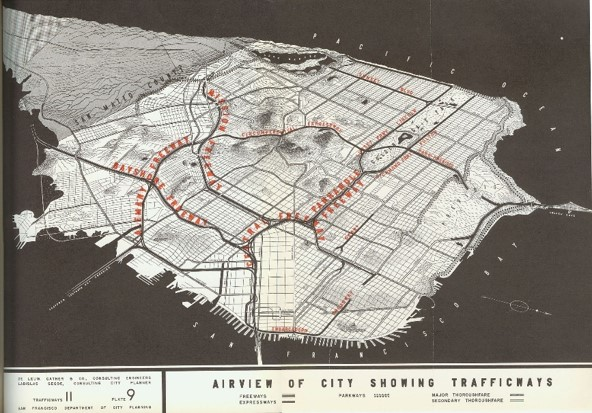
\includegraphics[height=0.3\textheight]{chp01_旧金山.jpg}
      \caption{1948年旧金山路网规划图}
    \end{figure}
  \end{column}
  \begin{column}{.6\textwidth}
    \begin{figure}\flushleft
      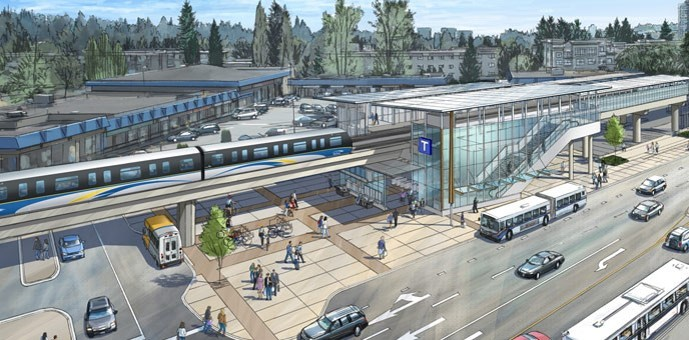
\includegraphics[height=0.3\textheight]{chp01_交通设计.jpg}
      \caption{城市公交站点交通设计图}
    \end{figure}
  \end{column}
\end{columns}
% \begin{figure}\centering
%   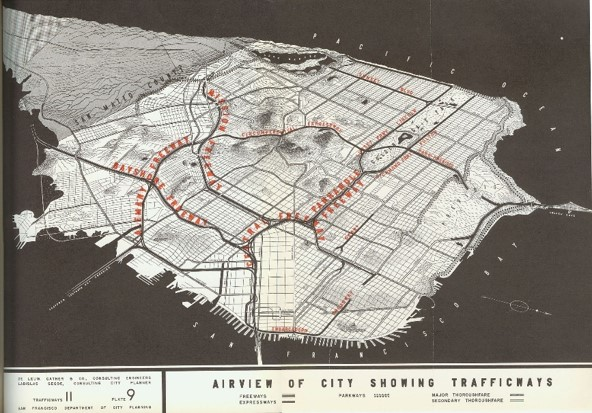
\includegraphics[width=0.6\textwidth]{chp01_旧金山.jpg}
%   \caption{1948年旧金山路网规划图}
% \end{figure}
\end{frame}

\begin{frame}[t]{\subsecname}
\begin{itemize}
\item \emphText{交通调查}是交通规划业务最主要的数据来源,并以此为依据建立分析模型推断规划方案
\item 国内一般\emphText{5--10年}进行一次城市居民出行调查,每次调查的时间长达数月甚至一年
\end{itemize}

\begin{figure}
  \centering
  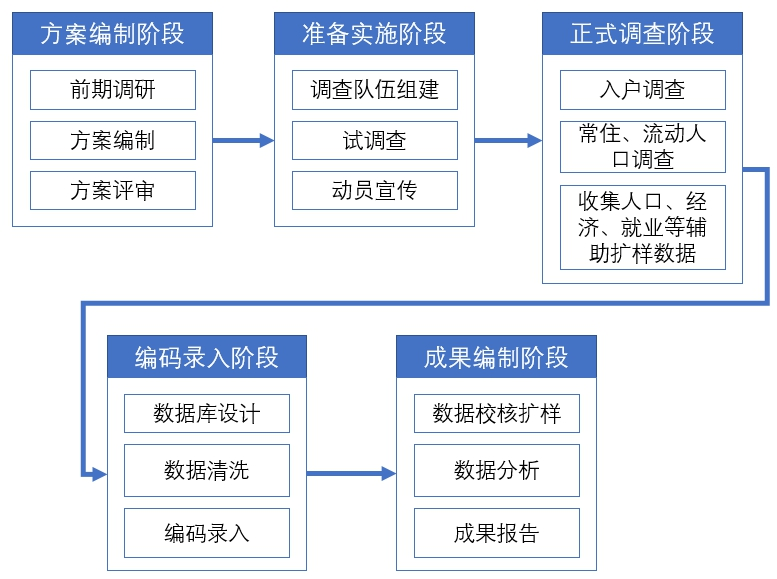
\includegraphics[width=0.65\textwidth]{chp01_交通调查.jpg}
  \caption{交通调查的一般流程}
\end{figure}
\end{frame}

\subsection{什么是大数据}

\begin{frame}[t]{\subsecname}
\begin{goodbox}{IBM公司对大数据的定义}
\begin{enumerate}\footnotesize
    \item Volume:海量的数据规模
    \item Velocity:快速的数据流转和动态的数据体系
    \item Variety:多样的数据类型
    \item Value:巨大的数据价值
    \item Veracity:数据的准确性和可信赖度
\end{enumerate}
\end{goodbox}

\begin{figure}
\begin{columns}
  \begin{column}{.5\textwidth}
      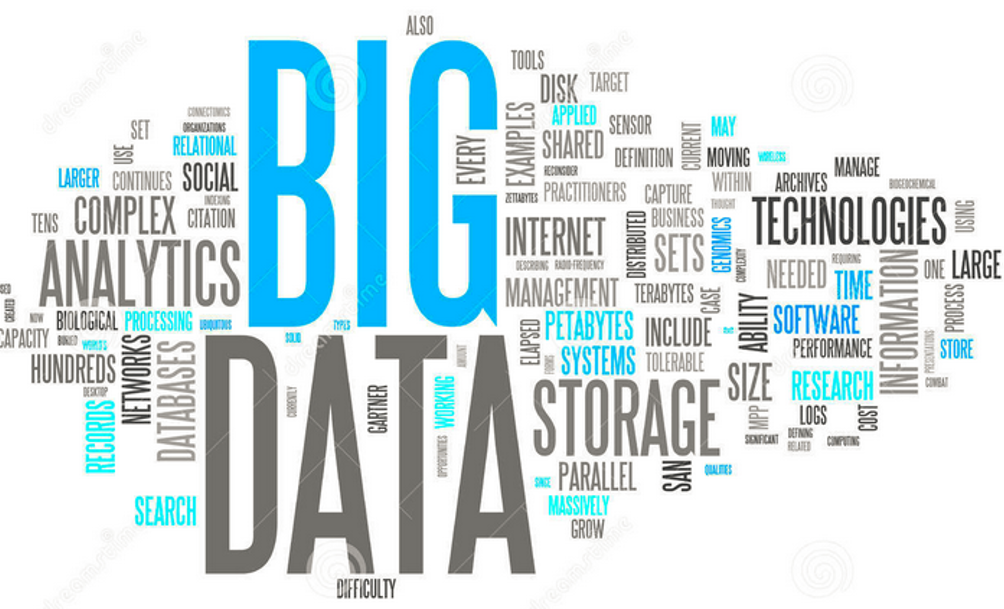
\includegraphics[height=0.35\textheight]{chp01_文字云.png}
  \end{column}
  \begin{column}{.5\textwidth}
      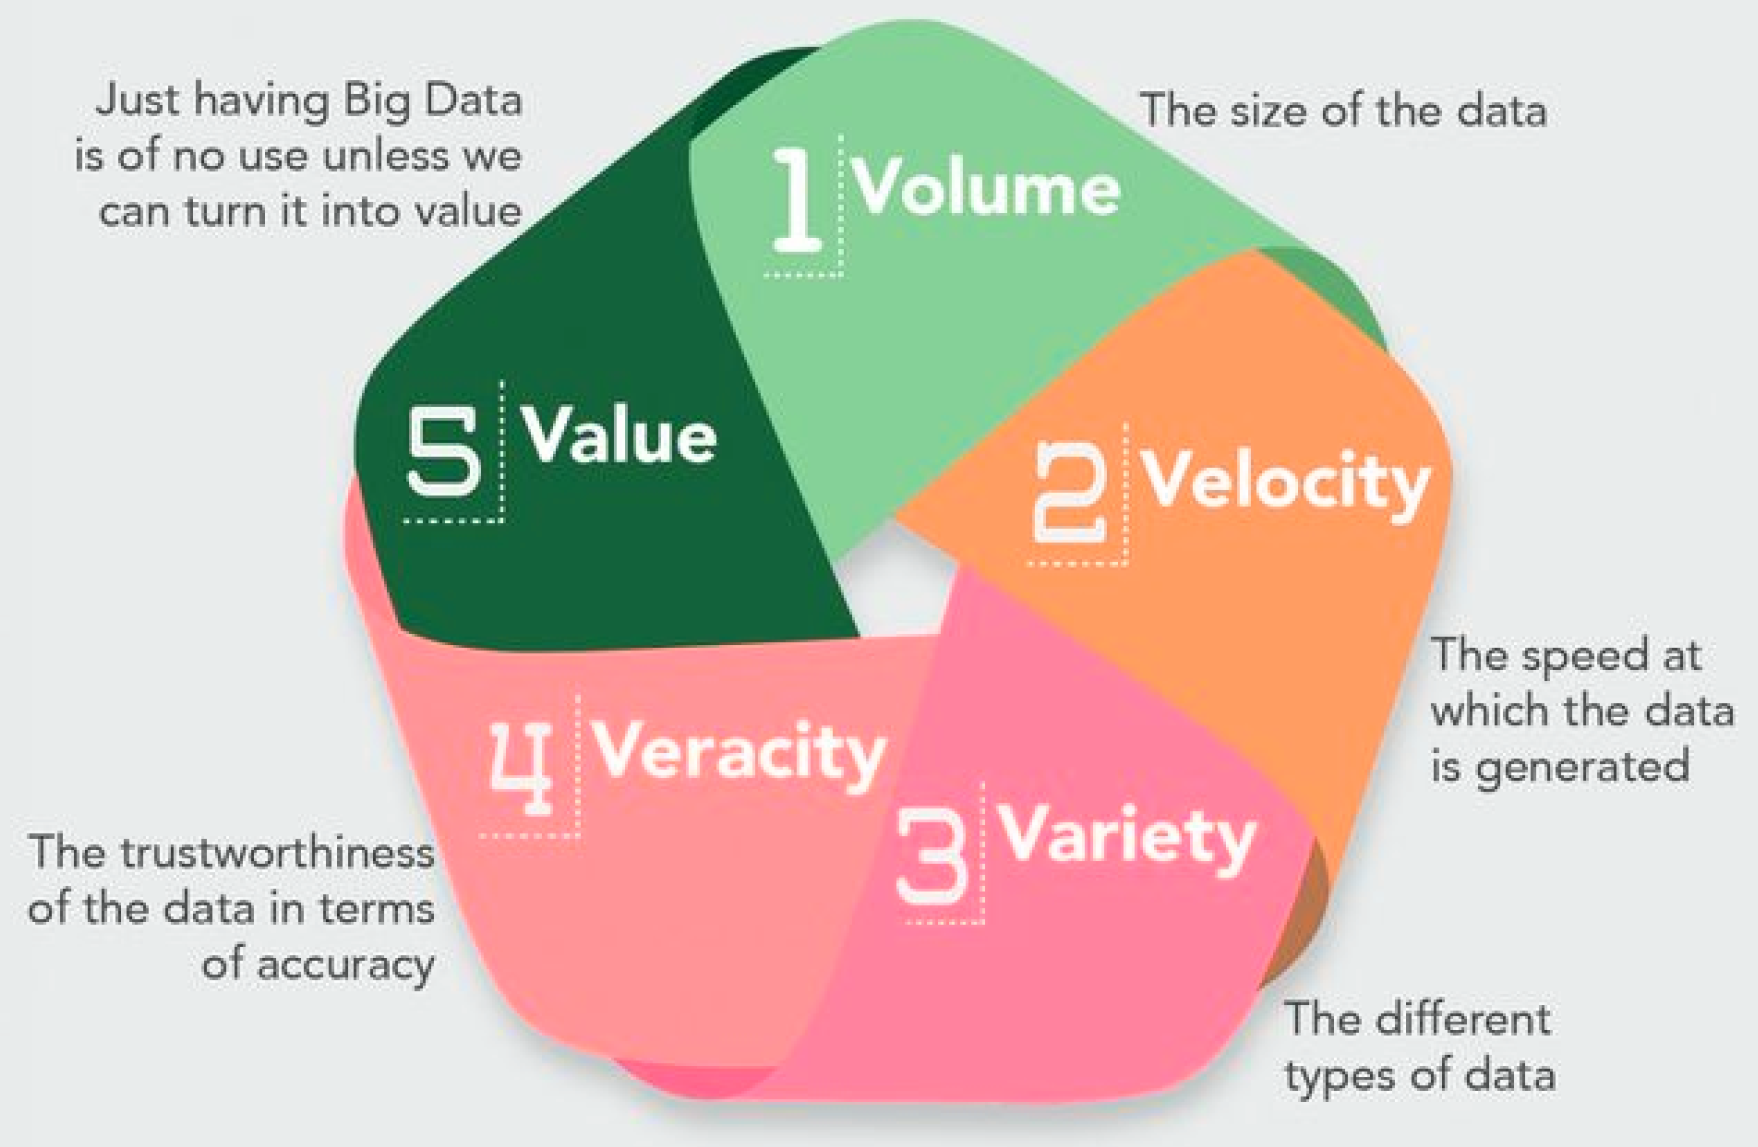
\includegraphics[height=0.35\textheight]{chp01_5V.png}
  \end{column}
\end{columns}
\caption{大数据的5V定义}
\end{figure}
\end{frame}

\begin{frame}[t]{\subsecname}
\begin{itemize}
\item<1-> 与传统数据相比,不仅体现在数据量巨大,更重要的是可以覆盖业务的近乎全部数据
\item<2-> 数据爆炸时代的必然产物
\item<3-> 商业公司进行的一场成功的营销 
\end{itemize}

\begin{overlayarea}{\textwidth}{\textheight}
  \begin{onlyenv}<4>
     \begin{columns}
       \begin{column}{.3\textwidth}
       \begin{figure}
         \centering 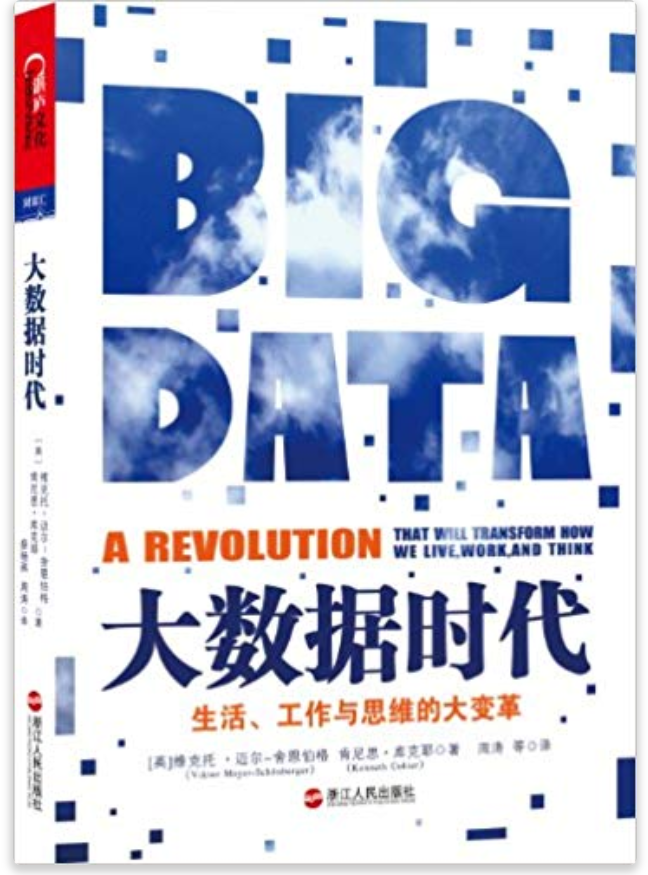
\includegraphics[width=\columnwidth]{chp01_bigdatabook.png}
       \end{figure}
       \end{column}
       \begin{column}{.7\textwidth}
      \begin{ornamentblock}
          \hspace*{2em}大数据是一场思维的颠覆:放弃对因果关系(为什么)的渴求,
而取而代之关注相关关系(是什么)。\\
          \rightline{\textemdash 维克托$\cdot$迈尔$\cdot$舍恩伯格}
      \end{ornamentblock}
       \end{column}
     \end{columns}
  \end{onlyenv}
\end{overlayarea}
\end{frame}

\subsection{大数据对规划编制的影响}

\begin{frame}[t]{\subsecname}
\begin{itemize}
\item<1-> 外部条件与时代背景
\pause
\begin{commonbox}{技术进步} 
随着计算机技术的发展,尤其是云计算和人工智能技术的进步,使得数据获取变得容易了许多,而且处理和分析的能力越来越强
\end{commonbox}
\pause 
\begin{commonbox}{经济转型} 
当前中国的经济正处于重要的转型时期,经济的发展模式、发展要素、发展路径等等都亟需转变,以适应现在的大环境
\end{commonbox}
\pause
\begin{commonbox}{社会转型} 
虽然我们的经济实现了快速发展,但社会矛盾出现越来越尖锐化的趋势
\end{commonbox}
\end{itemize}
\end{frame}

\begin{frame}[t]{\subsecname}
\begin{itemize}
\item 传统城市空间规划面临方法转型
\end{itemize}

\begin{commonbox}{规划转型} 
\begin{itemize} 
\item 传统时空间概念被重新定义,以空间研究和布局为核心内容的城市空间规划
面临着研究范式的转型和规划编制方法上的革新
\item 随着国内城市化进程的发展,规划面临的更多是城市的存量式发展,由粗放向集约进行转型,
对规划的精细化、定量化管理提出了要求
\end{itemize}
\end{commonbox}
\begin{figure}
  \centering
  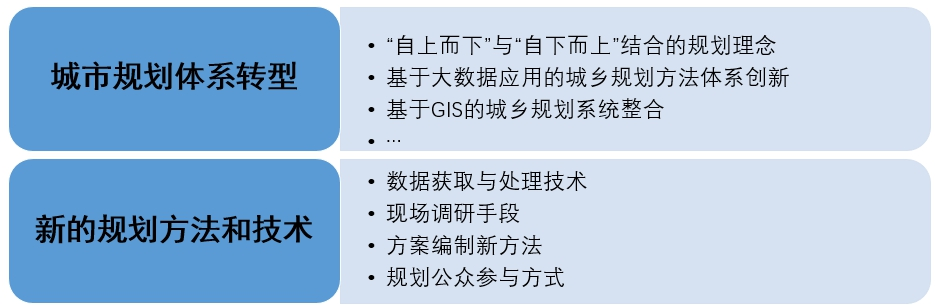
\includegraphics[width=0.85\textwidth]{chp01_规划转型.jpg}
  \caption{南京大学规划专业试行的学科教学改革方案}
\end{figure}
\end{frame}

\begin{frame}[t]{\subsecname}
\begin{itemize}
\item 大数据提供了认识和分析城市问题\emphText{新的思维和技术方法}
\item 大数据时代到来,可以让我们更清楚地了解和观察城市的发展、变化过程,同时也\emphText{使得规划过程变得透明可控};
\item 大数据技术强化了对规划过程的重视和科学化,尤其是对规划调研、空间分析、公共参与与空间协调规划、
空间预测和可视化等过程的科学把握,\emphText{有助于推动规划过程的科学化}
\end{itemize}
\begin{figure}
  \centering
  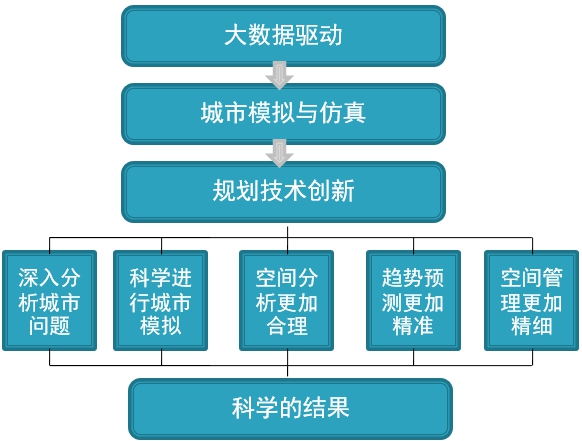
\includegraphics[width=0.55\textwidth]{chp01_数据驱动的城市规划.jpg}
  \caption{大数据驱动的规划决策评估架构}
\end{figure}
\end{frame}